\chapter{Communication protocol, state synchronization and future work}
\label{chap:proto}
This chapter is dedicated to the specification, design and implementation criteria of what will be referred to as the Distributed Group Creation Protocol (DGCP).
While in the previous chapters it has been suggested an algorithm for how groups can be formed, in this chapter the focus shall be on the technology and protocols required
to enable communication between access points, - and ultimately groups. There has already been done some work on the subject of access point communication over IP,
and previous work in the field of distributed consensus can be used to ensure synchronized group states. In this chapter these technologies will be covered and considered,
and finally a protocol sketch that stitches all required components together will be suggested. 


\section{Problem overview}
In chapter \ref{chap:clustering} we looked at an algorithm that enables cluster formation in a distributed environment where no node knows the complete layout of the surrounding networks.
A number of assumptions were made before we suggested an algorithm. Two of the assumptions encapsulated the three following problems:
\begin{itemize}
\item Direct contact between access points is possible
\item An underlying group communication protocol is in place
\item The state of a group is synchronized throughout all its members
\end{itemize}
In this chapter we look at technologies that can handle these issues to suggest an abstract architecture for a protocol that enables group creation in a distributed environment.

\section{Enabling technologies}
When designing a protocol that enables group communication, there is need for some some already well-researched theory and technology as a foundation. There are already enough
considerations to take when designing an architecture like this, and there is no need to reinvent the wheel where there is already done a good amount of research. 
Raft will be used for state synchronzation. Raft is a distributed consensus protocol and provides the equivalent degree of fault-tolerance as the Paxos \cite{lamport2001paxos} protocol family.
ResFi is a protocol used to enable communication over IP between adjacent access points. This section is dedicated to briefly introduce these protocols. 

\subsection{Distributed consensus with Raft}
Raft \cite{raftio} is a distributed consensus protocol designed with simplicity in mind. The creators of Raft designed it to be used for educational purposes. Traditionally, Paxos has been used to explain
distributed consensus, but Paxos has a complex design with extremely many different variations. Raft is now taught in courses all over the U.S, and their GitHub page includes to links
of implementations in a large amount of languages. As Raft has such a wide range of implementations and is an easy protocol to understand relative to its quite complicated relative, Paxos, 
we will suggest that Raft will be used to handle distributed consensus. 

\subsection{Why distributed consensus?}
Distributed consesus is required for the distributed group creation protocol for a couple of reasons, the most important two being:
\begin{itemize}
	\item Leader election for decision making
	\item	Synchronous data replication (makes sure all nodes have a consistent picture of the group, in-case leader goes down)
\end{itemize}

These reason are derived from the simple fact that there is no centralized controller to take decisions, so equally replicated data across all members node is required for all access
points to reach the same decisions about group membership. 

\subsection{What Raft can not help with}
Raft is not originally intended to run in a flexible environment where the amount of servers changes rapidly. Thus, Raft is not able to handle the group membership changes
after two groups merge, within the same Raft session. This is because there can be no consensus on past logs between nodes from different groups, as all groups will have different logs from before the merge. There is also no native Raft method to invoke native leader handover, so in the event of merge there would be two leaders. 

Another aspect that would be different from a traditional distributed consensus scenario, is the assumption that there are two main actors with different roles: servers and clients.
In distributed consensus, each server is supposed to have their own data, identical via data replication across across all the servers in the Raft session. The clients are the actor that requests 
changes on the data.

A traditional scenario is the banking example: a client could be a mini-bank issuing a withdrawal from a bank account. The servers would be all the banking servers making sure the new,
updated account balance is consistent no matter where money is withdrawn from. 

In the distributed group creation protocol all nodes running Raft are both servers and clients. They have to report new changes in the form of neighbours and signal strength values,
while also keeping a local, replicated copy of the state of the group.

\subsection{Access point communication with ResFi}
This subsection is dedicated to briefly describe how ResFi operates, and to cover why and how it is a protocol that can be taken advantage of in the Distributed Group Creation Protocol. 

ResFi is a protocol framework that supports creation of radio resource management in legacy residential networks. ResFi is intented to be used in  a chaotically deployed landscape of acccess points,
which is similar to the intentions of the group creation in this thesis. It enables the creation of secure point-to-point communication channel over IP through wired backhaul network. 
Point-to-point in this context means APs that are directly adjacant (or neighbouring APs as it has been referred to in the group creation chapter).
It also supports secure broadcast via n-hop communication. A brief account of the sequential steps of the ResFi standard mode of operation follows,
the more thorough explanation can be find in the ResFi paper \cite{resfi} under chapter \textit{IV. Detailed Specification}.

\begin{enumerate}
	\item When an AP ($a$) is booted, a symmetric group key is created, along with an RSA key-pair. 
	\item $a$ scans all 802.11 channels for neighbouring APs. For each AP it finds, $a$ sends out a probe request that contains its public IP and public RSA key. It also includes
		the symmetric group key. As a response to the probe request it receives a probe response containing the equivalent information for each neighbour. 
	\item When the exhchange has happened, $a$ subscribes to the publish sockets of all the neighbouring nodes using the IP received in step 2. Each neighbour in turn subscribes to $a$'s
		publish sockets as well. This makes it possible for each AP to broadcast messages to all subscribed neighbours,
		or create a unicast session key between one specific AP to enable secure and bidirectional unicast communication.
\end{enumerate}

ResFi has a north-bound framework API that lets application running on the AP use ResFi's features through an API, without doing direct modifications to the implementation. All communication happens
in the JSON-format. Table \ref{tab:resfapi} shows which functions are available in the north-bound API, original table also including the south-bound API functions can be found in \cite{resfi} table 1.

\begin{table}[h]
	\small
	\resizebox{\textwidth}{!}{%
		\begin{tabular}{|l|l|}
			\hline
			sendToNeighbor(ap\_id, message) & \makecell[l]{Sends a message to an ap with id ap\_id. Message is in JSON format.\\The message is encrypted using the symmetric unciast session key.} \\
			\hline
			sendToNeighbors(msg, TTL) & \makecell[l]{Sends a message to all neighbours.\\Will be flooded out to n-hop neighbours, where n = TTL.} \\
			\hline
			getNeighbour() & List all neighbour AP IDs \\
			\hline	
			regCallbacks(newMessage, newNode, nodeDC) & \makecell[l]{Registers callback functions for the events new message,\\new neighbour node, and node disconnected. } \\
			\hline
			registerNewApplication(name) & \makecell[l]{Registers a new application with ResFi.\\Names are used to separate different applications.}\\
			\hline
			getResFiCredentials(param) & \makecell[l]{If param is 1, it return the public IP of the AP,\\ and if param is 2 it returns the public RSA key}\\
			\hline
			usePrivateRSAKey(data, mode) & \makecell[l]{Uses RSA key on tjhe data. If the mode is 1, it computes\\the signature of the data, if mode is 2 it assumed the\\data is encrypted and
																									decrypts it with the key.} \\
			\hline
		\end{tabular}}
		\caption{ResFi north-bound API}
		\label{tab:resfapi}
\end{table}


\section{Protocol design}
This section outlines the architecture of a protocol that could facilitate group creation.

\subsection{Archictectural overview}
The protocol architecture we suggest here relies on 4 main components which can be seen in figure \ref{fig:dgcpoverview}.
In the figure the blue boxes signifies logic that has yet to be implemented, while grey boxes signifies the components that needs to pre-exist. The arrows
represents which of the components that has to communicate with each other. In the next few subsections we address the two blue compontents individually.


\begin{figure}
	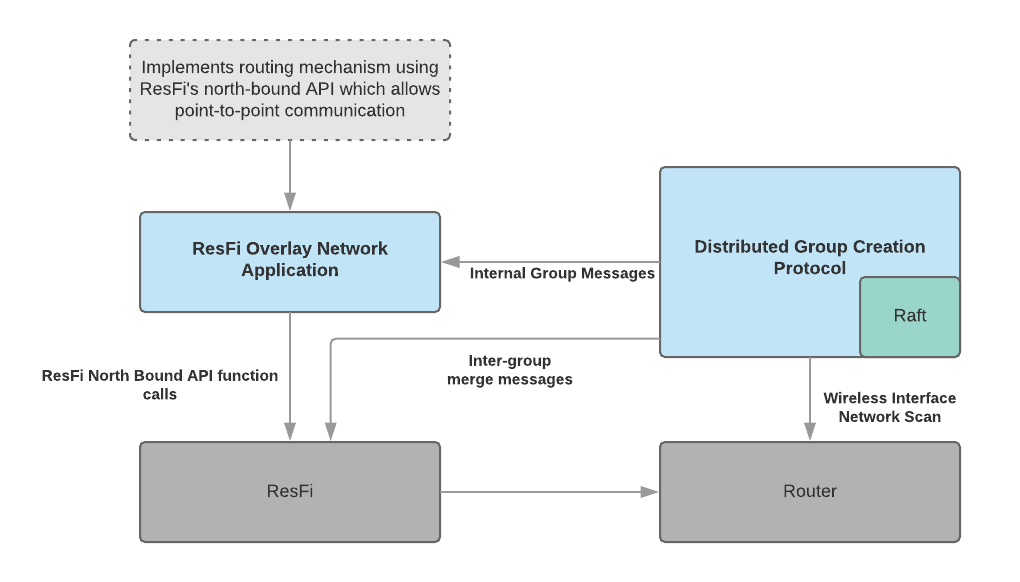
\includegraphics[width=\textwidth]{Images/dgcpoverview.png}
		\caption{Architectural overview of protocol components }%
		\label{fig:dgcpoverview}%
\end{figure}


\subsection{ResFi Overlay Network Application}
As made clear earlier, ResFi enables secure two-way communication between 1-hop neighbours, and broadcast messaging via n-hop neighbours. 
To enable secure two-way unicast communication throughout the group, an overlay network application can be built using the north-bound ResFi API. 
This means the overlay network application would have to use ResFi for point-to-point communication, and then implement its own routing mechanism
to relay messages from node to node, until the message reaches its destination. Let us look at the following suggested criteria for the ResFi Overlay Network Application:

\begin{itemize}
	\item Messages sent through the ResFi OverLay Network Application can only reach members of the group. If a message is requested for a node not inside the group,
		the message is not relayed.
  \item Should be used for all communication between nodes, like control messages, Raft log updates, etc., except for merge messages, which would have to happen across
		groups. 
	\item Uses IPv6 address to uniquely identify nodes  ???
\end{itemize}


\subsection{Distributed Group Creation Protocol}
This subsection is dedication to a suggested architectural overview of the Distributed Group Creation Protocol (DGCP). 
The protocol relies on the ability to directly interface with the access point radio, to execute and parse the results of the network scan. The protocol also
needs to be able to send message through the ResFi Overlay Network Applications to the rest of the group, as well as direct access to the ResFi north-bound API to be able to contact 1-hop
neighbours that are not in the group, to negotiate merges. 

The roles of a node running the protocol is illustrated in figure \ref{fig:dgcproles}. What follows is an account on the different services and functionalities the protocol
has to implement.  
\begin{itemize}
	\item Decide which nodes to merge with. 
	\item Negotiate merges with neighoburs not in the same group
	\item Incorporate Raft to ensure all nodes in the group know the entire group network topology 
\end{itemize}

\begin{figure}
	\centering
	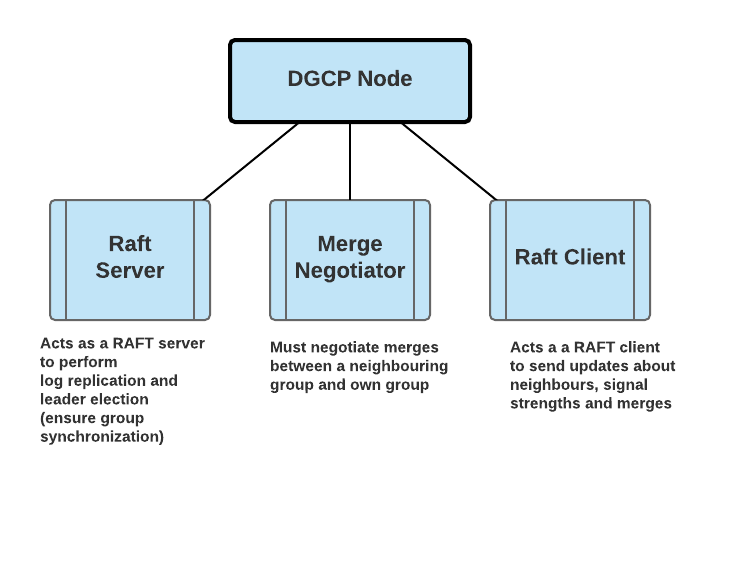
\includegraphics[width=8cm]{Images/dgcpnode.png}
		\caption{The roles of a DGCP Node }%
		\label{fig:dgcproles}%
\end{figure}



\subsubsection{Deciding which nodes to merge with}
Since the beginning of the thesis, the idea has been to let all nodes have the exact same information about the group state to calculate the same results. Deciding
which neighbouring groups to merge the group with is done by checking which nodes in the group has the most impactful neighbours. As all nodes in the group should share
the same information, all nodes will find the same result of which neighbour to merge with.
In the event that nodes in the group observe neighbours with exact equal signal strength, there will need to be implemented a deterministic way to decide which of the nodes would be chosen.
This could be as simple choosing the neighbours with the highest alphbetical order of the SSID. The important matter is that all nodes reach the same result of which group to merge with. 

\subsubsection{Negotiating merges via message passing}
We established that the protocol has to make sure all nodes in a group conclude which neighbour disturbs the most on their own.
For the sake of simplicity, we call this most disturbing neighbour $X$. $X$ is a member of group $G$. So now the nodes in the starting group knows it will attempt a merge with group $G$.
The node that lies physically closest to $X$ should be responsible for negotiating the merge.
We can be sure this node will be able to observe $X$ over its radio, and can then use direct ResFi uni-cast communication with this node. 

For the handling of merges themselves, there are probably several ways this can be executed. In this thesis we suggest the following way:
Node $N$ contacts is a part of a group $G$ that has identified node $X$ as the most disturbing node. Node $N$ will then contact the node issuing a \verb|merge request| message directly over ResFi.
The merge request contains the entire network topology of $G$. $X$ will then locally merge the nodes to see if it is valid according to the maximum size. If the merge is accepted, it replies with a \verb|merge accept|. 

The Distributed Group Creation Protcol uses the ResFi Overlay Network Application to communicate with the rest of the group. Group communication messages should include (but may not be limited to):
		\begin{itemize}
			\item Neighbour updates, e.g. a new access point appeared on the network scan of one of the routers, or significant signal strength value changes
			\item Raft log updates, heartbeats, vote requests, and vote messages
			\item Merge attempts 
			\end{itemize}


\subsubsection{Preventing duplicate merge attempts}
To prevent a group from repeatedely attempting to merge with another group we suggest that a hashing the member datatru

\section{Future Work}
\begin{itemize}
	\item Assessment of the ResFi overlay network application, the protocol, modification and implementation
	\item Testing group creation using the clustering algorithms
	\item Security evaluation

\end{itemize}


